\documentclass[a4paper]{article}

\usepackage{array,amsmath,amssymb,rotating,graphicx}

\input{tutorial_style.texinc}

\newcommand{\mat}[1]{{\tt >> #1} \\}
\newcommand{\com}[1]{{\tt #1}}

%\newcommand{\tit}[1]{{\noindent \bf #1 \\}}
\newcommand{\tab}{\hspace{1em}}

% for MATH MODE
\newcommand{\trn}{^{\mathsf T}} % transposition
\newcommand{\xv}{\ensuremath\mathbf{x}}  % vector x
\newcommand{\muv}{\ensuremath\boldsymbol{\mu}}  % vector mu
\newcommand{\Sm}{\ensuremath\boldsymbol{\Sigma}}  % matrix Sigma
\newcommand{\Tm}{\ensuremath\boldsymbol{\Theta}}  % matrix Sigma
\newcommand{\Rf}{\ensuremath\mathbb{R}}


\setlength{\hoffset}{-1in}
\setlength{\voffset}{-1in}

\setlength{\topskip}{0cm}
\setlength{\headheight}{0cm}
\setlength{\headsep}{0cm}

\setlength{\textwidth}{16cm}
\setlength{\evensidemargin}{2.5cm}
\setlength{\oddsidemargin}{2.5cm}

\setlength{\textheight}{24cm}
\setlength{\topmargin}{2.5cm}
\setlength{\headheight}{0.5cm}
\setlength{\headsep}{0.5cm}

%\pagestyle{fancyplain}


\begin{document}

%%%%%%%%%%%%%%%%%%%%%%%%% Make Title %%%%%%%%%%%%%%%%%%%%%%%%%%%%%%

\author{\small Barbara Resch (minor changes by Erhard Rank)\\
Signal Processing and Speech Communication Laboratory\\
Inffeldgasse 16c/II\\
phone 873--4436}
\date{}

\MakeTutorialTitle{Gaussian Statistics and Unsupervised Learning}

%%%%%%%%%%%%%%%%%%%%%%%%%%%%%%%%%%%%%%%%%%%%%%%%%%%%%%%%%%%%%%%%%%%

\subsubsection*{Abstract}
This tutorial presents the properties of the Gaussian probability
density function. Subsequently, supervised and unsupervised pattern
recognition methods are treated. Supervised classification algorithms
are based on a labeled data set. The knowledge about the class
membership of this training data set is used for the classification of
new samples. Unsupervised learning methods establish clusters from an
unlabeled training data set.  Clustering algorithms such as the
$K$-means, the EM (expectation-maximization) algorithm, and the
Viterbi-EM algorithm are presented.

\subsubsection*{Usage} To make full use of this tutorial you have to
\begin{enumerate}
  
\item download the file
  \HREF{http://www.igi.tugraz.at/lehre/CI/tutorials/Gaussian.zip}
  {\texttt{Gaussian.zip}} which contains this tutorial \html{in
    printable format (\href{Gaussian.pdf}{PDF} and
    \href{Gaussian.ps.gz}{ps.gz})} and the accompanying Matlab
  programs.

\item Unzip \texttt{Gaussian.zip} which will generate a
  subdirectory named \texttt{Gaussian/matlab} where you can find
  all the Matlab programs.
  
\item Add the path \texttt{Gaussian/matlab} to the matlab search path,
  for example with a command like
  \verb#addpath('C:\Work\Gaussian\matlab')# if you are using a Windows
  machine, or by using a command like
  \verb#addpath('/home/jack/Gaussian/matlab')# if you are on a
  Unix/Linux machine.

\end{enumerate}

\subsubsection*{Sources}
This tutorial is based on 

% ftp://ftp.idiap.ch/pub/sacha/labs/labman1.pdf
% or http://www.ai.mit.edu/~murphyk/Software/HMM/labman2.pdf
\begin{itemize}
\item EPFL lab notes 
  ``Introduction to Gaussian Statistics and Statistical Pattern
    Recognition'' by Herv\'e Bourlard, Sacha Krstulovi\'c, and Mathew
  Magimai-Doss.
\end{itemize}


\html{
\subsubsection*{Contents}
}


\section{Gaussian statistics}
%%%%%%%%%
%%%%%%%%%

%%%%%%%%%
\subsection{Samples from a Gaussian density}
\label{samples}
%%%%%%%%%

\subsubsection*{Useful formulas and definitions:}\label{sec:gausspdf}
\begin{itemize}
  
\item The {\em Gaussian probability density function (pdf)} for the
  $d$-dimensional random variable $\xv \circlearrowleft {\cal
    N}(\muv,\Sm)$ (i.e., variable $\xv \in \Rf^d$ following the
  Gaussian, or Normal, probability law) is given by:
  \begin{equation}
    \label{eq:gauss}
    g_{(\muv,\Sm)}(\xv) = \frac{1}{\sqrt{2\pi}^d
      \sqrt{\det\left(\Sm\right)}} \, e^{-\frac{1}{2} (\xv-\muv)\trn
      \Sm^{-1} (\xv-\muv)}
  \end{equation}
  where $\muv$ is the mean vector and $\Sm$ is the covariance matrix.
  $\muv$ and $\Sm$ are the {\em parameters} of the Gaussian
  distribution.
  
\item The mean vector $\muv$ contains the mean values of each
  dimension, $\mu_i = E(x_i)$, with $E(x)$ being the \emph{expected
    value} of $x$.
  
\item All of the variances $c_{ii}$ and covariances $c_{ij}$ are
  collected together into the covariance matrix $\Sm$ of dimension
  $d\times d$:

\begin{equation*}
  \Sm =
  \left[
    \begin{array}{*{4}{c}}
      c_{11} & c_{12} & \cdots & c_{1n} \\
      c_{21} & c_{22} & \cdots & c_{2n} \\
      \vdots & \vdots & \ddots & \vdots \\
      c_{n1} & c_{n2} & \cdots & c_{nn} \\
    \end{array}
  \right]
\end{equation*}

The covariance $c_{ij}$ of two components $x_i$ and $x_j$ of $\xv$
measures their tendency to vary together, i.e., to co-vary,
\[ c_{ij} = E\left((x_i-\mu_i)\trn\,(x_j-\mu_j)\right).\]
If two components $x_i$ and $x_j$, $i\ne j$, have zero covariance
$c_{ij} = 0$ they are {\em orthogonal} in the statistical sense, which
transposes to a geometric sense (the expectation is a scalar product
of random variables; a null scalar product means orthogonality).  If
all components of $\xv$ are mutually orthogonal the covariance matrix
has a diagonal form.


\item $\sqrt{\Sm}$ defines the {\em standard deviation} of the random
  variable $\xv$. Beware: this square root is meant in the {\em matrix
    sense}.
  
\item If $\xv \circlearrowleft {\cal N}(\mathbf{0},\mathbf{I})$ ($\xv$
  follows a normal law with zero mean and unit variance; $\mathbf{I}$
  denotes the identity matrix), and if $\mathbf{y} = \muv +
  \sqrt{\Sm}\,\xv$, then $\mathbf{y} \circlearrowleft {\cal
    N}(\muv,\Sm)$.

\end{itemize}


\subsubsection{Experiment:}
Generate samples $X$ of $N$ points, $X=\{\xv_1,
\xv_2,\ldots,\xv_N\}$, with $N=10000$, coming from a 2-dimensional
Gaussian process that has mean
\[
\muv = \left[ \begin{array}{c} 730 \\ 1090 \end{array} \right]
\]
and variance
\begin{itemize}
%%%%%
\item
  8000 for both dimensions ({\em spherical process}) (sample $X_1$):
  \[
  \Sm_1 = \left[ \begin{array}{cc}
      8000 & 0 \\
      0    & 8000
    \end{array} \right]
  \]
%%%%%
\item
  expressed as a {\em diagonal} covariance matrix (sample $X_2$):
  \[
  \Sm_2 = \left[ \begin{array}{cc}
      8000 & 0 \\
      0    & 18500
    \end{array} \right]
  \]
%%%%%
\item
  expressed as a {\em full} covariance matrix (sample $X_3$):
  \[
  \Sm_3 = \left[ \begin{array}{cc}
      8000 & 8400 \\
      8400 & 18500
    \end{array} \right]
  \]
%%%%%
\end{itemize}
%
Use the function \com{gausview} (\com{>> help gausview}) to plot the
results as clouds of points in the 2-dimensional plane, and to view the
corresponding 2-dimensional probability density functions (pdfs) in 2D and
3D.

\subsubsection*{Example:}
\mat{N = 10000;}
\mat{mu = [730 1090]; sigma\_1 = [8000 0; 0 8000];}
\mat{X1 = randn(N,2) * sqrtm(sigma\_1) + repmat(mu,N,1);}
\mat{gausview(X1,mu,sigma\_1,'Sample X1');}
%
Repeat for the two other variance matrices $\Sm_2$ and $\Sm_3$.
Use the radio buttons to switch the plots on/off. Use the ``view''
buttons to switch between 2D and 3D. Use the mouse to rotate the plot
(must be enabled in \com{Tools} menu: \com{Rotate 3D}, or by the
$\circlearrowleft$ button).

\subsubsection*{Questions:}
By simple inspection of 2D views of the data and of the corresponding
pdf contours, how can you tell which sample corresponds to a spherical
process (as the sample $X_1$), which sample corresponds to a process
with a diagonal covariance matrix (as $X_2$), and which to a process
with a full covariance matrix (as $X_3$)?

\subsubsection*{Find the right statements:}
\begin{itemize}
\item[$\Box$] In process 1 the first and the second component of the
  vectors $\xv_i$ are independent.
  
\item[$\Box$] In process 2 the first and the second component of the
  vectors $\xv_i$ are independent.
  
\item[$\Box$] In process 3 the first and the second component of the
  vectors $\xv_i$ are independent.
  
\item[$\Box$] If the first and second component of the vectors $\xv_i$
  are independent, the cloud of points and the pdf contour has the
  shape of a circle.
  
\item[$\Box$] If the first and second component of the vectors $\xv_i$
  are independent, the cloud of points and pdf contour has to be
  elliptic with the principle axes of the ellipse aligned with the
  abscissa and ordinate axes.
  
\item[$\Box$] For the covariance matrix $\Sm$ the elements have to
  satisfy $c_{ij} = c_{ji}$.
  
\item[$\Box$] The covariance matrix has to be positive definite
  ($\xv\trn \Sm\, \xv \ge 0$). (If yes, what happens if not? Try it
  out in \textsc{Matlab}).
\end{itemize}

%\pagebreak
%%%%%%%%%
\subsection{Gaussian modeling: Mean and variance of a sample}
%%%%%%%%%

We will now estimate the parameters $\muv$ and $\Sm$ of the Gaussian
models from the data samples.

\subsubsection*{Useful formulas and definitions:}
\begin{itemize}
\item Mean estimator: $\displaystyle \hat{\muv} = \frac{1}{N}
  \sum_{i=1}^{N} \xv_i$
\item Unbiased covariance estimator: $\displaystyle \hat{\Sm} =
  \frac{1}{N-1} \; \sum_{i=1}^{N} (\xv_i-\muv)\trn (\xv_i-\muv) $
\end{itemize}

\subsubsection{Experiment:}
Take the sample $X_3$ of 10000 points generated from ${\cal
  N}(\muv,\Sm_3)$. Compute an estimate $\hat{\muv}$ of its mean and an
estimate $\hat{\Sm}$ of its variance:
\begin{enumerate}
\item with all the available points \hspace{1cm}$\hat{\muv}_{(10000)}
  =$\hspace{3.5cm}$\hat{\Sm}_{(10000)} =$ \vspace{0.8cm}
\item with only 1000 points \hspace{1.95cm}$\hat{\muv}_{(1000)}
  =$\hspace{3.7cm}$\hat{\Sm}_{(1000)} =$ \vspace{0.8cm}
\item with only 100 points \hspace{2.2cm}$\hat{\muv}_{(100)}
  =$\hspace{3.9cm}$\hat{\Sm}_{(100)} =$ \vspace{0.8cm}
\end{enumerate}
Compare the estimated mean vector $\hat{\muv}$ to the original mean
vector $\muv$ by measuring the Euclidean distance that separates them.
Compare the estimated covariance matrix $\hat{\Sm}$ to the original
covariance matrix $\Sm_3$ by measuring the matrix 2-norm of their
difference (the norm $\|\mathbf{A}-\mathbf{B}\|_2$ constitutes a
measure of similarity of two matrices $\mathbf{A}$ and $\mathbf{B}$;
use {\sc Matlab}'s \com{norm} command).

\subsubsection{Example:}
In the case of 1000 points (case 2.): \\
\mat{X = X3(1:1000,:);}
\mat{N = size(X,1)}
\mat{mu\_1000 = sum(X)/N}
\textit{--or--}\\
\mat{mu\_1000 = mean(X)}
\mat{sigma\_1000 = (X - repmat(mu\_1000,N,1))' * (X - repmat(mu\_1000,N,1)) / (N-1)}
\textit{--or--}\\
\mat{sigma\_1000 = cov(X)}

\noindent
\mat{\% Comparison of means and covariances:}
\mat{e\_mu =  sqrt((mu\_1000 - mu) * (mu\_1000 - mu)')}
\mat{\% (This is the Euclidean distance between mu\_1000 and mu)}
\mat{e\_sigma = norm(sigma\_1000 - sigma\_3)}
\com{>> \% (This is the 2-norm of the difference between sigma\_1000 and sigma\_3)}

\subsubsection{Question:}
When comparing the estimated values $\hat{\muv}$ and $\hat{\Sm}$ to
the original values of $\muv$ and $\Sm_3$ (using the Euclidean
distance and the matrix 2-norm), what can you observe?

\subsubsection*{Find the right statements:}
\begin{itemize}
\item[$\Box$] An accurate mean estimate requires more points than an
  accurate variance estimate.
\item[$\Box$] It is very important to have enough training examples to
  estimate the parameters of the data generation process accurately.
\end{itemize}


%\pagebreak

\subsection{Likelihood of a sample with respect to a Gaussian model}
\label{sec:likelihood}

In the following we compute the likelihood of a sample point $\xv$,
and the joint likelihood of a series of samples $X$ for a given model
$\Tm$ with one Gaussian.  The likelihood will be used in the formula
for classification later on (sec.~\ref{sec:classification}).

\subsubsection*{Useful formulas and definitions:}
\begin{itemize}
\item {\em Likelihood}: the likelihood of a sample point $\xv_i$ given
  a data generation model (i.e., given a set of parameters $\Tm$ for
  the model pdf) is the value of the pdf $p(\xv_i|\Tm)$ for that
  point. In the case of Gaussian models $\Tm = (\muv,\Sm)$, this
  amounts to the evaluation of equation~\ref{eq:gauss}.
\item {\em Joint likelihood}: for a set of independent identically
  distributed (i.i.d.) samples, say $X = \{\xv_1, \xv_2, \ldots, \xv_N
  \}$, the joint (or total) likelihood is the product of the
  likelihoods for each point. For instance, in the Gaussian case:
  \begin{equation}
    \label{eq:joint-likelihood}
    p(X|\Tm) =
    \prod_{i=1}^{N} p(\xv_i|\Tm) =
    \prod_{i=1}^{N} p(\xv_i|\muv,\Sm) =
    \prod_{i=1}^{N} g_{(\muv,\Sm)}(\xv_i)
  \end{equation}
\end{itemize}


\subsubsection{Question:}
Why do we might want to compute the {\em log-likelihood} rather than
the simple {\em likelihood}?
\\

Computing the log-likelihood turns the product into a sum:
\[
p(X|\Tm) = \prod_{i=1}^{N} p(\xv_i|\Tm) \quad \Leftrightarrow \quad
\log p(X|\Tm) = \log \prod_{i=1}^{N} p(\xv_i|\Tm) = \sum_{i=1}^{N}
\log p(\xv_i|\Tm)
\]

In the Gaussian case, it also avoids the computation of the exponential:
\begin{eqnarray}
  \label{eq:loglikely}
  p(\xv|\Tm) & = & \frac{1}{\sqrt{2\pi}^d \sqrt{\det\left(\Sm\right)}}
  \, e^{-\frac{1}{2} (\xv-\muv)\trn \Sm^{-1} (\xv-\muv)} \nonumber \\
  \log p(\xv|\Tm) & = &
  \frac{1}{2} \left[-d \log \left( 2\pi \right)
    -  \log \left( \det\left(\Sm\right) \right)
    -  (\xv-\muv)\trn \Sm^{-1} (\xv-\muv)\right]
\end{eqnarray}
Furthermore, since $\log(x)$ is a monotonically growing function, the
log-likelihoods have the same relations of order as the likelihoods
\[
p(x|\Tm_1) > p(x|\Tm_2) \quad \Leftrightarrow \quad
\log p(x|\Tm_1) > \log p(x|\Tm_2),
\]
so they can be used directly for classification.

\subsubsection*{Find the right statements:}
We can further simplify the computation of the log-likelihood in
eq.~\ref{eq:loglikely} for classification by
\begin{itemize}
\item[$\Box$] dropping the division by two: $\frac{1}{2}
  \left[\ldots\right]$,
\item[$\Box$] dropping term $d\log \left( 2\pi \right)$,
\item[$\Box$] dropping term $\log \left( \det\left(\Sm\right)
  \right)$,
\item[$\Box$] dropping term $(\xv-\muv)\trn \Sm^{-1} (\xv-\muv)$,
\item[$\Box$] calculating the term $\log \left( \det\left(\Sm\right)
  \right)$ in advance.
\end{itemize}

\medskip
\noindent
We can drop term(s) because:
\begin{itemize}
\item[$\Box$] The term(s) are independent of $\muv$.
\item[$\Box$] The terms are negligible small.
\item[$\Box$] The term(s) are independent of the classes.
\end{itemize}

\noindent As a summary, log-likelihoods use simpler computation and are readily
usable for classification tasks.


\subsubsection{Experiment:}
Given the following 4 Gaussian models $\Tm_i = (\muv_i,\Sm_i)$
\begin{center}
\begin{tabular}{ccc}
${\cal N}_1: \; \Tm_1 = \left(
\left[\begin{array}{c}730 \\ 1090\end{array}\right],
\left[\begin{array}{cc}8000 & 0 \\ 0 & 8000\end{array}\right]
\right)$ & \hspace{2cm} &
${\cal N}_2: \; \Tm_2 = \left(
\left[\begin{array}{c}730 \\ 1090\end{array}\right],
\left[\begin{array}{cc}8000 & 0 \\ 0 & 18500\end{array}\right]
\right)$ \\[2em]
${\cal N}_3: \; \Tm_3 = \left(
\left[\begin{array}{c}730 \\ 1090\end{array}\right],
\left[\begin{array}{cc}8000 & 8400 \\ 8400 & 18500\end{array}\right]
\right)$ & \hspace{2cm} &
${\cal N}_4: \; \Tm_4 = \left(
\left[\begin{array}{c}270 \\ 1690\end{array}\right],
\left[\begin{array}{cc}8000 & 8400 \\ 8400 & 18500\end{array}\right]
\right)$
\end{tabular}
\end{center}
\vspace{0.5em} compute the following {log-likelihoods} for the whole sample
$X_3$ (10000 points):


\[
\log p(X_3|\Tm_1),\; \log p(X_3|\Tm_2),\; \log p(X_3|\Tm_3),\;
\text{and}\; \log p(X_3|\Tm_4).
\]

\subsubsection{Example:}
\mat{N = size(X3,1)}
\mat{mu\_1 = [730 1090]; sigma\_1 = [8000 0; 0 8000];}
\mat{logLike1 = 0;}
\mat{for i = 1:N;}
\com{logLike1 = logLike1 + (X3(i,:) - mu\_1) * inv(sigma\_1) * (X3(i,:) - mu\_1)';} \\
\com{end;} \\
\mat{logLike1 =  - 0.5 * (logLike1 + N*log(det(sigma\_1)) + 2*N*log(2*pi))}

\noindent Note: Use the function \com{gausview} to compare the
relative positions of the models ${\cal N}_1$, ${\cal N}_2$, ${\cal
  N}_3$ and ${\cal N}_4$ with respect to the data set $X_3$, e.g.:
\\
%
\mat{mu\_1 = [730 1090]; sigma\_1 = [8000 0; 0 8000];}
\mat{gausview(X3,mu\_1,sigma\_1,'Comparison of X3 and N1');}
%
\vspace{-\baselineskip}
\subsubsection*{Question:}
Of ${\cal N}_1$, ${\cal N}_2$, ${\cal N}_3$ and ${\cal N}_4$, which
model ``explains'' best the data $X_3$?  Which model has the highest
number of parameters (with non-zero values)?  Which model would you
choose for a good compromise between the number of parameters and the
capacity to accurately represent the data?


%%%%%%%%%
%%%%%%%%%
\section{Statistical pattern recognition}
%%%%%%%%%
%%%%%%%%%

%%%%%%%%%
\subsection{A-priori class probabilities}
\label{sec:apriori}
%%%%%%%%%
\subsubsection{Experiment:}
Load data from file ``vowels.mat''. This file contains a database of
2-dimensional samples of speech features in the form of formant
frequencies (the first and the second spectral formants, $[F_1,F_2]$).
The formant frequency samples represent features that would be
extracted from the speech signal for several occurrences of the vowels
/a/, /e/, /i/, /o/, and /y/\footnote{/y/ is the phonetic symbol for
  ``\"u''}.  They are grouped in matrices of size $N\times2$, where
each of the $N$ lines contains the two formant frequencies for one
occurrence of a vowel.

Supposing that the whole database covers adequately an imaginary
language made only of /a/'s, /e/'s, /i/'s, /o/'s, and /y/'s, compute
the probability $P(q_k)$ of each class $q_k$, $k \in
\{\text{/a/},\text{/e/},\text{/i/},\text{/o/},\text{/y/}\}$. Which is
the most common and which the least common phoneme in our imaginary
language?

\subsubsection{Example:}
\mat{clear all; load vowels.mat; whos}
\mat{Na = size(a,1); Ne = size(e,1); Ni = size(i,1); No = size(o,1); Ny = size(y,1);}
\mat{N = Na + Ne + Ni + No + Ny;}
\mat{Pa = Na/N}
\mat{Pi = Ni/N}
etc.


%%%%%%%%
\subsection{Gaussian modeling of classes}
\label{gaussmod}
%%%%%%%%%

\subsubsection*{Experiment:}
Plot each vowel's data as clouds of points in the 2D plane. Train the
Gaussian models corresponding to each class (use directly the
\com{mean} and \com{cov} commands). Plot their contours (use directly
the function \com{plotgaus(mu,sigma,color)} where \com{color =
  [R,G,B]}).

\subsubsection{Example:}
\mat{plotvow; \% Plot the clouds of simulated vowel features}
(Do not close the figure obtained, it will be used later on.) \\
Then compute and plot the Gaussian models: \\
\mat{mu\_a = mean(a);}
\mat{sigma\_a = cov(a);}
\mat{plotgaus(mu\_a,sigma\_a,[0 1 1]);}
\mat{mu\_e = mean(e);}
\mat{sigma\_e = cov(e);}
\mat{plotgaus(mu\_e,sigma\_e,[0 1 1]);}
etc.


%%%%%%%%%%%%%%%%%%
%%%%%%%%%
\subsection{Bayesian classification}
\label{sec:classification}
%%%%%%%%%

We will now find how to classify a feature vector $\xv_i$ from a data
sample (or several feature vectors $X$) as belonging to a certain
class $q_k$.

\subsubsection*{Useful formulas and definitions:}
\begin{itemize}
\item {\em Bayes' decision rule}:
  \[
  X \in q_k \quad \mbox{if} \quad P(q_k|X,\Tm) \geq P(q_j|X,\Tm),
  \quad\forall j \neq k
  \]
  This formula means: given a set of classes $q_k$, characterized by a
  set of known parameters in model $\Tm$, a set of one or more speech
  feature vectors $X$ (also called {\em observations}) belongs to the
  class which has the highest probability once we actually know (or
  ``see'', or ``measure'') the sample $X$. $P(q_k|X,\Tm)$ is therefore
  called the {\em a posteriori probability}, because it depends on
  having seen the observations, as opposed to the {\em a priori}
  probability $P(q_k|\Tm)$ which does not depend on any observation
  (but depends of course on knowing how to characterize all the
  classes $q_k$, which means knowing the parameter set $\Tm$).
  
\item For some classification tasks (e.g. speech recognition), it is
  practical to resort to {\em Bayes' law}, which makes use of {\em
    likelihoods} (see sec.~\ref{sec:likelihood}), rather than trying
  to directly estimate the posterior probability $P(q_k|X,\Tm)$.
  Bayes' law says:
  \begin{equation}
    \label{eq:decision-rule}
    P(q_k|X,\Tm) = \frac{p(X|q_k,\Tm)\; P(q_k|\Tm)}{p(X|\Tm)}
  \end{equation}
  where $q_k$ is a class, $X$ is a sample containing one or more
  feature vectors and $\Tm$ is the parameter set of all the class
  models.
  
\item The speech features are usually considered equi-probable:
  $p(X|\Tm)=\text{const.}$ (uniform prior distribution for $X$).
  Hence, $P(q_k|X,\Tm)$ is proportional to $p(X|q_k,\Tm) P(q_k|\Tm)$
  for all classes:
  \[
  P(q_k|X,\Tm) \propto p(X|q_k,\Tm)\; P(q_k|\Tm), \quad \forall k
  \]

\item Once again, it is more convenient to do the computation in the
  $\log$ domain:
  \begin{equation}
    \label{eq:log-decision-rule}
    \log P(q_k|X,\Tm) \propto \log p(X|q_k,\Tm) + \log P(q_k|\Tm)
  \end{equation}
\end{itemize}

In our case, $\Tm$ represents the set of \emph{all} the means $\muv_k$
and variances $\Sm_k$, $k \in
\{\text{/a/},\text{/e/},\text{/i/},\text{/o/},/u/\}$ of our data
generation model.  $p(X|q_k,\Tm)$ and $\log p(X|q_k,\Tm)$ are the
joint likelihood and joint log-likelihood
(eq.~\ref{eq:joint-likelihood} in section~\ref{sec:likelihood}) of the
sample $X$ with respect to the model $\Tm$ for class $q_k$ (i.e., the
model with parameter set $(\muv_k,\Sm_k)$).

The probability $P(q_k|\Tm)$ is the a-priori class probability for the
class $q_k$. It defines an absolute probability of occurrence for the
class $q_k$. The a-priori class probabilities for our phoneme classes
have been computed in section~\ref{sec:apriori}.


\subsubsection{Experiment:}
Now, we have modeled each vowel class with a Gaussian pdf (by
computing means and variances), we know the probability $P(q_k)$ of
each class in the imaginary language (sec.~\ref{sec:apriori}), which
we assume to be the correct a priori probabilities $P(q_k|\Tm)$ for
each class given our model $\Tm$.  Further we assume that the speech
\emph{features} $\xv_i$ (as opposed to speech {\em classes} $q_k$) are
equi-probable\footnote{Note, that -- also for not equi-probable
  features -- finding the most probable class $q_k$ according to
  eq.~\ref{eq:decision-rule} does not depend on the denominator
  $p(X|\Tm)$, since $p(X|\Tm)$ is independent of $q_k$!}.

What is the most probable class $q_k$ for each of the formant pairs
(features) $\xv_i=[F_1,F_2]\trn$ given in the table below?  Compute
the values of the functions $f_k(\xv_i)$ for our model $\Tm$ as the
right-hand side of eq.~\ref{eq:log-decision-rule}: $f_k(\xv_i) = \log
p(\xv_i|q_k,\Tm) + \log P(q_k|\Tm)$, proportional to the log of the
posterior probability of $\xv_i$ belonging to class $q_k$.

\medskip
\noindent
\begin{center}
  \renewcommand{\arraystretch}{1.5}
  \setlength{\tabcolsep}{0.12in}
  \begin{tabular}{|c|c|c|c|c|c|c|c|} \hline
    i & \small$\xv_i=[F_1,F_2]\trn$ &
    \small $f_{\text{/a/}}(\xv_i)$ &
    \small $f_{\text{/e/}}(\xv_i)$ &
    \small $f_{\text{/i/}}(\xv_i)$ &
    \small $f_{\text{/o/}}(\xv_i)$ &
    \small $f_{\text{/y/}}(\xv_i)$ & 
    Most prob.\ class $q_k$ \\
    \hline
    1 & $[400,1800]\trn$ & & & & & & \\ \hline
    2 & $[400,1000]\trn$ & & & & & & \\ \hline
    3 & $[530,1000]\trn$ & & & & & & \\ \hline
    4 & $[600,1300]\trn$ & & & & & & \\ \hline
    5 & $[670,1300]\trn$ & & & & & & \\ \hline
    6 & $[420,2500]\trn$ & & & & & & \\ \hline
  \end{tabular}
\end{center}

\subsubsection{Example:}
Use function \com{gloglike(point,mu,sigma)} to compute the
log-likelihoods $\log p(\xv_i|q_k,\Tm)$.  Don't forget to add the log
of the prior probability $P(q_k|\Tm)$!
E.g., for the feature set $x_1$ and class /a/ use\\
\com{>> gloglike([400,1800],mu\_a,sigma\_a) + log(Pa)}



\bigskip
%%%%%%%%%
\subsection{Discriminant surfaces}
\label{sec:discr}
%%%%%%%%%
For the Bayesian classification in the last section we made use of the
\emph{discriminant functions} $f_k(\xv_i) = \log p(\xv_i|q_k,\Tm) +
\log P(q_k|\Tm)$ to classify data points $\xv_i$.  This corresponds to
establishing \emph{discriminant surfaces} of dimension $d-1$ in the
vector space for $\xv$ (dimension $d$) to separate regions for the
different classes.

\subsubsection*{Useful formulas and definitions:}
\begin{itemize}
\item {\em Discriminant function}: a set of functions $f_k(\xv)$ allows
  to classify a sample $\xv$ into $k$ classes $q_k$ if:
  \[
  \xv \in q_k \quad \Leftrightarrow \quad f_k(\xv,\Tm_k) \geq f_l(\xv,\Tm_l),
  \quad \forall l \neq k
  \]
  In this case, the $k$ functions $f_k(\xv)$ are called discriminant
  functions.
\end{itemize}

The a-posteriori probability $P(q_k|\xv_i)$ that a sample $\xv_i$
belongs to class $q_k$ is itself a discriminant function:
\begin{eqnarray*}
  \xv \in q_k 
  & \Leftrightarrow & P(q_k|\xv_i) \geq P(q_l|\xv_i),\quad \forall l \neq k \\
  & \Leftrightarrow & p(\xv_i|q_k)\; P(q_k) \geq p(\xv_i|q_l)\; P(q_l),\quad
  \forall l \neq k \\
  & \Leftrightarrow & \log p(\xv_i|q_k)+\log P(q_k) \geq \log
  p(\xv_i|q_l)+\log P(q_l),\quad \forall l \neq k
\end{eqnarray*}

As in our case the samples $\xv$ are two-dimensional vectors, the
discriminant surfaces are one-dimensional, i.e., lines at equal values
of the discriminant functions for two distinct classes.

\subsubsection{Experiment:}
%%%%%%%%%%%%
\begin{figure}
\centerline{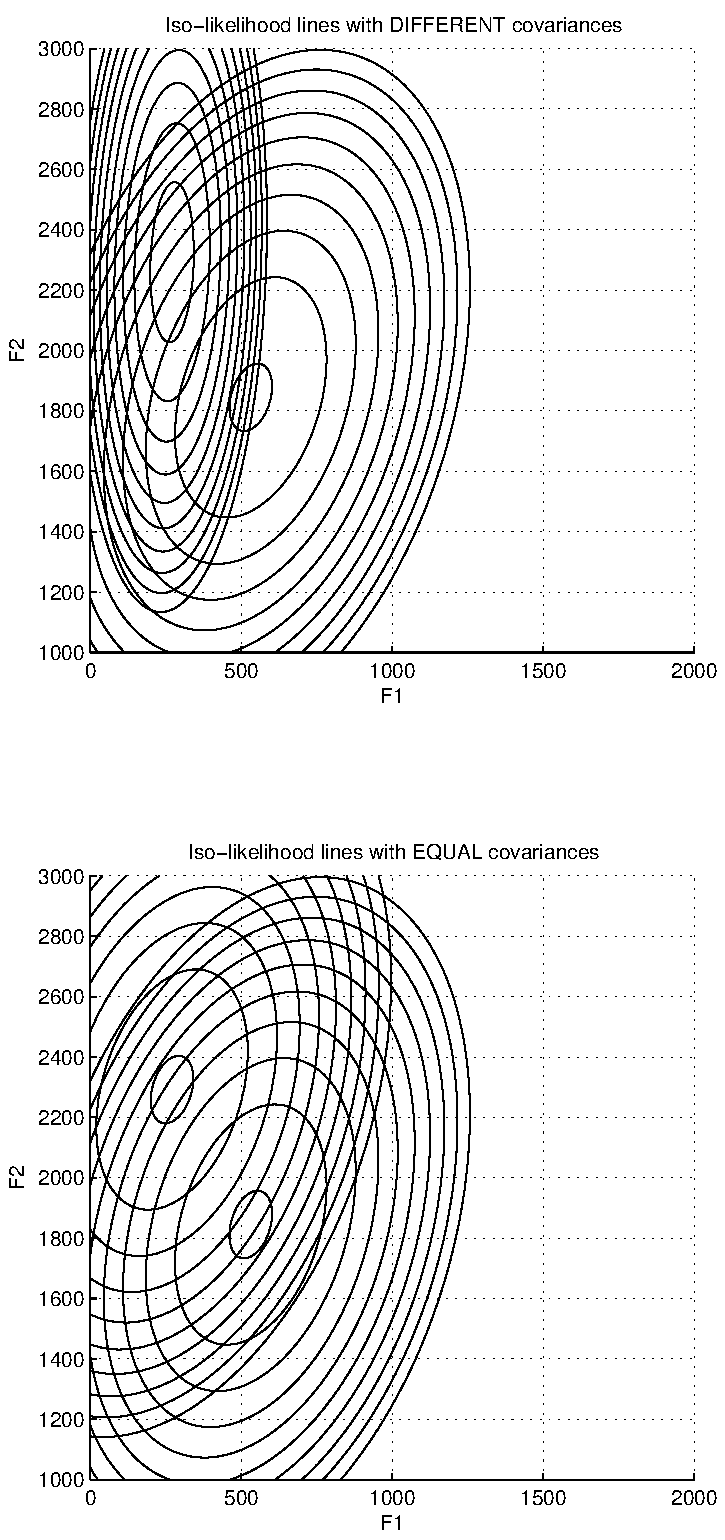
\includegraphics[height=0.95\textheight]{iso}}
\caption{\label{iso}Iso-likelihood lines for the Gaussian pdfs
  ${\cal N}(\muv_{\text{/i/}},\Sm_{\text{/i/}})$ and ${\cal
    N}(\muv_{\text{/e/}},\Sm_{\text{/e/}})$ (top), and ${\cal
    N}(\muv_{\text{/i/}},\Sm_{\text{/e/}})$ and ${\cal
    N}(\muv_{\text{/e/}},\Sm_{\text{/e/}})$ (bottom).}
\end{figure}
%%%%%%%%%%%%
The iso-likelihood lines for the Gaussian pdfs ${\cal
  N}(\muv_{\text{/i/}},\Sm_{\text{/i/}})$ and ${\cal
  N}(\muv_{\text{/e/}},\Sm_{\text{/e/}})$, which we used before to
model the class /i/ and the class /e/, are plotted in
figure~\ref{iso}, first graph. On the second graph in
figure~\ref{iso}, the iso-likelihood lines for ${\cal
  N}(\muv_{\text{/i/}},\Sm_{\text{/e/}})$ and ${\cal
  N}(\muv_{\text{/e/}},\Sm_{\text{/e/}})$ (two pdfs with the
\emph{same} covariance matrix $\Sm_{\text{/e/}}$) are represented.  

On these figures, use a colored pen to join the intersections of the
level lines that correspond to equal likelihoods.  Assume that the
highest iso-likelihood lines (smallest ellipses) are of the same
height. (You can also use \com{isosurf} in {\sc Matlab} to create a
color plot.)

\subsubsection{Question:}
What is the nature of the surface that separates class /i/ from class
/e/ when the two models have {\em different} variances? Can you
explain the origin of this form?

What is the nature of the surface that separates class /i/ from class
/e/ when the two models have the {\em same} variances? Why is it
different from the previous discriminant surface?
\\

Show that in the case of two Gaussian pdfs with \emph{equal covariance
  matrices}, the separation between class 1 and class 2 does not
depend upon the covariance $\Sm$ any more.
\\

\tab As a summary, we have seen that Bayesian classifiers with
Gaussian data models separate the classes with combinations of
parabolic surfaces. If the covariance matrices of the models are
equal, the parabolic separation surfaces become simple hyper-planes.



\bigskip
%%%%%%%%%
%%%%%%%%%



\section{Unsupervised training}
\label{unsup}
%%%%%%%%%
%%%%%%%%%
In the previous section, we have computed the models for classes /a/,
/e/, /i/, /o/, and /y/ by knowing a-priori which training samples
belongs to which class (we were disposing of a {\em labeling} of the
training data). Hence, we have performed a {\em supervised training}
of the Gaussian models.  Now, suppose that we only have unlabeled
training data that we want to separate in several classes (e.g., 5
classes) without knowing a-priori which point belongs to which class.
This is called {\em unsupervised training}. Several algorithms are
available for that purpose, among them: the $K$-means, the EM
(Expectation-Maximization), and the Viterbi-EM algorithm.


%
All these algorithms are characterized by the following components:
\begin{itemize}
\item a set of models for the classes $q_k$ (not necessarily
  Gaussian), defined by a parameter set $\Tm$ (means, variances,
  priors,...);
\item a measure of membership, telling to which extent a data point
``belongs'' to a model;
\item a ``recipe'' to update the model parameters as a function of the
  membership information.
\end{itemize}
The measure of membership usually takes the form of a distance measure
or the form of a measure of probability. It replaces the missing
labeling information to permit the application of standard parameter
estimation techniques.  It also defines implicitly a global criterion
of ``goodness of fit'' of the models to the data, e.g.:
\begin{itemize}
\item in the case of a distance measure, the models that are closer to
  the data characterize it better;
\item in the case of a probability measure, the models with a larger
  likelihood for the data explain it better.
\end{itemize}

\begin{latexonly}
Table~\ref{algos} summarizes the components of the algorithms that
will be studied in the following experiments. More detail will be
given in the corresponding subsections.

%\pagebreak
%\newpage
%\pagestyle{empty}
\newcommand{\PBS}[1]{\let\temp=\\#1\let\\=\temp}
\newcommand{\RR}{\PBS\raggedright\hspace{0pt}}
\newcommand{\RL}{\PBS\raggedleft\hspace{0pt}}
\newcommand{\CC}{\PBS\centering\hspace{0pt}}

\begin{sidewaystable}[p]
  %\setlength{\arrayrulewidth}{1.2pt}
  \setlength{\tabcolsep}{0.05in}
  \renewcommand{\arraystretch}{2.2}
  %\hspace{-1.5em}
  \begin{tabular}{|>{\RR}m{5.2em}|>{\RR}m{7.3em}|>{\CC}m{21em}|>{\RR}m{22.5em}|>{\CC}m{8em}|}
    \hline
    \centering\bf Algorithm &
    \centering\bf Parameters &
    \bf Membership measure &
    \centering\bf Update method &
    \bf Global criterion \\ \hline
                                %
    $K$-means    &
    $\bullet$ mean $\muv_k$ &
    Euclidean distance \linebreak
    \[d_k(\xv_n)= \sqrt{(\xv_n-\muv_k)\trn(\xv_n-\muv_k)}\] \linebreak
    (or the square of it)
    &
    Find the points closest to $q_k^{(i)}$, then:

    \medskip
    $\bullet$ $\muv_{k}^{(i+1)}$ = mean of the points closest to $q_k^{(i)}$ &
    Least squares \\ 
    \hline
    %
    % Kmeans w/ \linebreak Mahalanobis distance &
    % $\bullet$ mean $\muv_k$ \linebreak
    % $\bullet$ variance $\Sm_k$ &
    % Mahalanobis distance, \linebreak (Weighted Euclidean distance)
    % \[d_k(x_n)= \sqrt{(x_n-\muv_k)\trn\Sm_k^{-1}(x_n-\muv_k)}\]
    % &
    % Find the points closest to $q_k^{(i)}$, then:

    % \medskip
    % $\bullet$ $\muv_{k}^{(i+1)}$ = mean of the points closest to $q_k^{(i)}$

    % \medskip
    % $\bullet$ $\Sm_{k}^{(i+1)}$ = variance of the points closest to $q_k^{(i)}$ &
    % Minimal \linebreak spread of the data \linebreak (in a Mahalanobis distance sense) \\ \hline
    %
    Viterbi-EM &
    $\bullet$ mean $\muv_k$ \linebreak
    $\bullet$ variance $\Sm_k$ \linebreak
    $\bullet$ priors $P(q_k|\Tm)$
    &
    Posterior probability
    \[
    d_k(\xv_n) = P(q_k|\xv_n,\Tm)
    \]
    \footnotesize
    \[
    \propto \frac{1}{\sqrt{2\pi}^d \sqrt{\det\left(\Sm_k\right)}}
    \, e^{-\frac{1}{2} (\xv_n-\muv_k)\trn \Sm_k^{-1} (\xv_n-\muv_k)}
    \cdot P(q_k|\Tm)
    \]
    \normalsize
    &
    Do Bayesian classification of each data point, then:

    \medskip
    $\bullet$ $\muv_{k}^{(i+1)}$ = mean of the points belonging to $q_k^{(i)}$

    \medskip
    $\bullet$ $\Sm_{k}^{(i+1)}$ = variance of the points belonging to $q_k^{(i)}$

    \medskip
    $\bullet$ $P(q_k^{(i+1)}|\Tm^{(i+1)})$ = number of training points
    belonging to $q_k^{(i)}$ / total number of training points
    &
    Maximum likelihood \\ \hline
                                %
    EM &
    $\bullet$ mean $\muv_k$ \linebreak
    $\bullet$ variance $\Sm_k$ \linebreak
    $\bullet$ priors $P(q_k|\Tm)$ &
    Posterior probability
    \[
    d_k(\xv_n) = P(q_k|\xv_n,\Tm)
    \]
    \footnotesize
    \[
    \propto \frac{1}{\sqrt{2\pi}^d \sqrt{\det\left(\Sm_k\right)}}
    \, e^{-\frac{1}{2} (\xv_n-\muv_k)\trn \Sm_k^{-1} (\xv_n-\muv_k)}
    \cdot P(q_k|\Tm)
    \]
    \normalsize
    &
    Compute $P(q_k^{(i)}|\xv_n,\Tm^{(i)})$ (soft classification), then:

    \medskip
    $\bullet$ $\muv_{k}^{(i+1)} = \frac{\sum_{n=1}^{N} x_n P(q_k^{(i)}|\xv_n,\Tm^{(i)})}
    {\sum_{n=1}^{N} P(q_k^{(i)}|\xv_n,\Tm^{(i)})} $

    \medskip
    $\bullet$ $\Sm_{k}^{(i+1)} = \frac{\sum_{n=1}^{N} P(q_k^{(i)}|\xv_n,\Tm^{(i)})
      (\xv_n - \muv_k^{(i+1)})(\xv_n - \muv_k^{(i+1)})\trn }
    {\sum_{n=1}^{N} P(q_k^{(i)}|\xv_n,\Tm^{(i)})} $

    \medskip
    $\bullet$ $P(q_k^{(i+1)}|\Tm^{(i+1)}) = \frac{1}{N} \sum_{n=1}^{N} P(q_k^{(i)}|\xv_n,\Tm^{(i)}) $ &
    Maximum likelihood \\ \hline
  \end{tabular}

  \caption{\label{algos}Characteristics of some usual unsupervised
    clustering algorithms.}
\end{sidewaystable}
%
\end{latexonly}

%%%%%%%%%
%\newpage
%\pagestyle{fancyplain}
\subsection{$K$-means algorithm}
%%%%%%%%%
\subsubsection*{Synopsis of the algorithm:}
\begin{itemize}
\item Start with $K$ initial prototypes $\muv_k$, $k=1,\ldots,K$.
\item {\bf Do}:
  \begin{enumerate}
  \item For each data-point $\xv_n$, $n=1,\ldots,N$, compute the squared
    Euclidean distance from the $k^{\text{th}}$ prototype:
    \begin{eqnarray}
      \label{eq:dist}
      d_k(\xv_n) & = & \, \left\| \xv_n - \muv_k \right\|^2 \nonumber \\
      & = & (\xv_n-\muv_k)\trn(\xv_n-\muv_k)   \nonumber
    \end{eqnarray}
  \item Assign each data-point $\xv_n$ to its \emph{closest prototype}
    $\muv_k$, i.e., assign $\xv_n$ to the class $q_k$ if
    \[
    d_k(\xv_n) \, < \, d_l(\xv_n), \qquad \forall l \neq k
    \]
    {\em Note}: using the squared Euclidean distance for the
    classification gives the same result as using the true Euclidean
    distance, since the square root is a monotonically growing
    function. But the computational load is obviously smaller when the
    square root is dropped.
\item Replace each prototype with the mean of the data-points assigned to
  the corresponding class;
\item Go to 1.
\end{enumerate}

\item {\bf Until}: no further change occurs.
\end{itemize}

The global criterion for the present case is
\[
    J = \sum_{k=1}^{K} \sum_{\xv_n \in q_k} d_k(\xv_n)
\]
and represents the total squared distance between the data and the models
they belong to. This criterion is locally minimized by the algorithm.

% Alternately, the Euclidean distance used in step 1. can be replaced by the
% Mahalanobis distance, belonging to the class of weighted Euclidean
% distances:
% \[
%   d_k(x_n)= \sqrt{(x_n-\muv_k)\trn\Sm_k^{-1}(x_n-\muv_k)}
% \]
% where $\Sm_k$ is the covariance of the points associated with the class
% $q_k$.

% After the convergence of the algorithm, the final clusters of points may be
% used to make Gaussian models since we dispose of means and variances.


\subsubsection*{Experiment:}
Use the $K$-means explorer utility:
\begin{verbatim}
 KMEANS K-means algorithm exploration tool

   Launch it with KMEANS(DATA,NCLUST) where DATA is the matrix
   of observations (one observation per row) and NCLUST is the
   desired number of clusters.

   The clusters are initialized with a heuristic that spreads
   them randomly around mean(DATA) with standard deviation
   sqrtm(cov(DATA)).

   If you want to set your own initial clusters, use
   KMEANS(DATA,MEANS) where MEANS is a cell array containing
   NCLUST initial mean vectors.

   Example: for two clusters
     means{1} = [1 2]; means{2} = [3 4];
     kmeans(data,means);

\end{verbatim}

%\pagebreak

Launch \com{kmeans} with the data sample \com{allvow}, which was part
of file \com{vowels.mat} and gathers all the simulated vowels data. Do
several runs with different cases of initialization of the algorithm:
\begin{enumerate}
\item 5 initial clusters determined according to the default heuristic;
\item initial \com{MEANS} values equal to some data points;
\item initial \com{MEANS} values equal to $\{\muv_{\text{/a/}},
  \muv_{\text{/e/}}, \muv_{\text{/i/}}, \muv_{\text{/o/}},
  \muv_{\text{/y/}}\}$.
\end{enumerate}
Iterate the algorithm until its convergence. Observe the evolution of the
cluster centers, of the data-points attribution chart and of the total
squared Euclidean distance. (It is possible to zoom these plots: left
click inside the axes to zoom $2\times$ centered on the point under the
mouse; right click to zoom out; click and drag to zoom into an area; double
click to reset the figure to the original). %Observe the mean and variance
% values found after the convergence of the algorithm.
Observe the mean values found after the convergence of the algorithm.


\subsubsection*{Example:}
\mat{kmeans(allvow,5);}
- or - \\
\mat{means =  \{ mu\_a, mu\_e, mu\_i, mu\_o, mu\_y \};}
\mat{kmeans(allvow,means);}
Enlarge the window, then push the buttons, zoom etc.
After the convergence, use:\\
\mat{for k=1:5, disp(kmeans\_result\_means\{k\}); end}
to see the resulting means.


\subsubsection*{Think about the following question:}
\begin{enumerate}
\item Does the final solution depend on the initialization of the
  algorithm?
\item Describe the evolution of the total squared Euclidean distance.
\item What is the nature of the discriminant surfaces corresponding to
  a minimum Euclidean distance classification scheme?
\item Is the algorithm suitable for fitting Gaussian clusters?
\end{enumerate}


%%%%%%%%%
\subsection{Viterbi-EM algorithm for Gaussian clustering}
%%%%%%%%%
\subsubsection*{Synopsis of the algorithm:}
\begin{itemize}
\item Start from $K$ initial Gaussian models ${\cal N}(\muv_{k},\Sm_{k}),
\; k=1\ldots K$, characterized by the set of parameters $\Tm$ (i.e., the
set of all means and variances $\muv_k$ and $\Sm_k$, $k=1\ldots K$). Set
the initial prior probabilities $P(q_k)$ to $1/K$.
\item {\bf Do}:
\begin{enumerate}
\item Classify each data-point using Bayes' rule.

This step is equivalent to having a set $Q$ of boolean hidden variables
that give a labeling of the data by taking the value 1 (belongs) or 0 (does
not belong) for each class $q_k$ and each point $\xv_n$. The value of $Q$
that maximizes $p(X,Q|\Tm)$ precisely tells which is the most probable
model for each point of the whole set $X$ of training data.

Hence, each data point $\xv_n$ is assigned to its most probable
cluster $q_k$.
\item Update the parameters ($i$ is the iteration index):
\begin{itemize}
\item update the means:
    \[
    \muv_{k}^{(i+1)} = \mbox{mean of the points belonging to } q_k^{(i)}
    \]
\item update the variances:
    \[
    \Sm_{k}^{(i+1)} = \mbox{variance of the points belonging to } q_k^{(i)}
    \]
\item update the priors:
    \[
    P(q_k^{(i+1)}|\Tm^{(i+1)}) = \frac{\mbox{number of training points
        belonging to } q_k^{(i)} }{\mbox{total number of training points}}
    \]
\end{itemize}
\item Go to 1.
\end{enumerate}
\item {\bf Until}: no further change occurs.
\end{itemize}
The global criterion in the present case is
\begin{eqnarray*}
  {\cal L}(\Tm) &=& \sum_{X} P(X|\Tm) \;=\; \sum_{Q} \sum_{X} p(X,Q|\Tm) \\
  &=& \sum_{k=1}^{K} \sum_{\xv_n \in q_k} \log p(\xv_n|\Tm_k),
\end{eqnarray*}
and represents the joint likelihood of the data with respect to the models
they belong to. This criterion is locally maximized by the algorithm.


\subsubsection*{Experiment:}
Use the Viterbi-EM explorer utility:
\begin{verbatim}
 VITERB Viterbi version of the EM algorithm

   Launch it with VITERB(DATA,NCLUST) where DATA is the matrix
   of observations (one observation per row) and NCLUST is the
   desired number of clusters.

   The clusters are initialized with a heuristic that spreads
   them randomly around mean(DATA) with standard deviation
   sqrtm(cov(DATA)). Their initial covariance is set to cov(DATA).

   If you want to set your own initial clusters, use
   VITERB(DATA,MEANS,VARS) where MEANS and VARS are cell arrays
   containing respectively NCLUST initial mean vectors and NCLUST
   initial covariance matrices. In this case, the initial a-priori
   probabilities are set equal to 1/NCLUST.

   To set your own initial priors, use VITERB(DATA,MEANS,VARS,PRIORS)
   where PRIORS is a vector containing NCLUST a priori probabilities.

   Example: for two clusters
     means{1} = [1 2]; means{2} = [3 4];
     vars{1} = [2 0;0 2]; vars{2} = [1 0;0 1];
     viterb(data,means,vars);

\end{verbatim}
Launch \com{viterb} with the dataset \com{allvow}. Do several runs
with different initializations of the algorithm:
\begin{enumerate}
\item 5 initial clusters determined according to the default heuristic;
\item initial \com{MEANS} values equal to some data points, and some
  random \com{VARS} values (try for instance \com{cov(allvow)} for all
  the classes);
\item the initial \com{MEANS}, \com{VARS} and \com{PRIORS} values
  found by the $K$-means algorithm.
\item initial \com{MEANS} values equal to $\{\muv_{\text{/a/}},
  \muv_{\text{/e/}}, \muv_{\text{/i/}}, \muv_{\text{/o/}},
  \muv_{\text{/y/}}\}$, \com{VARS} values equal to \linebreak
  $\{\Sm_{\text{/a/}}, \Sm_{\text{/e/}}, \Sm_{\text{/i/}},
  \Sm_{\text{/o/}}, \Sm_{\text{/y/}}\}$, and \com{PRIORS} values
  equal to
  $[P_{\text{/a/}},P_{\text{/e/}},P_{\text{/i/}},P_{\text{/o/}},P_{\text{/y/}}]$;
\item initial \com{MEANS} and \com{VARS} values chosen by yourself.
\end{enumerate}
Iterate the algorithm until it converges. Observe the evolution of the
clusters, of the data points attribution chart and of the total
likelihood curve. Observe the mean, variance and priors values found
after the convergence of the algorithm. Compare them with the values
computed in section~\ref{gaussmod} (using supervised training).


\subsubsection*{Example:}
\mat{viterb(allvow,5);}
- or - \\
\mat{means =  \{ mu\_a, mu\_e, mu\_i, mu\_o, mu\_y \};}
\mat{vars = \{ sigma\_a, sigma\_e, sigma\_i, sigma\_o, sigma\_y \};}
\mat{viterb(allvow,means,vars);}
Enlarge the window, then push the buttons, zoom, etc.
After convergence, use:\\
\mat{for k=1:5, disp(viterb\_result\_means\{k\}); end}
\mat{for k=1:5, disp(viterb\_result\_vars\{k\}); end}
\mat{for k=1:5, disp(viterb\_result\_priors(k)); end}
to see the resulting means, variances and priors.


\subsubsection*{Question:}
\begin{enumerate}
\item Does the final solution depend on the initialization of the
algorithm?
\item Describe the evolution of the total likelihood. Is it monotonic?
\item In terms of optimization of the likelihood, what does the final
solution correspond to?
\item What is the nature of the discriminant surfaces corresponding to the
Gaussian classification?
\item Is the algorithm suitable for fitting Gaussian clusters?
\end{enumerate}




%%%%%%%%%
\subsection{EM algorithm for Gaussian clustering}
%%%%%%%%%
\subsubsection*{Synopsis of the algorithm:}
\begin{itemize}
\item Start from K initial Gaussian models ${\cal N}(\muv_{k},\Sm_{k}),
  \; k=1\ldots K$, with equal priors set to $P(q_k) = 1/K$.
\item {\bf Do}:
\begin{enumerate}
\item {\bf Estimation step}: compute the probability
  $P(q_k^{(i)}|\xv_n,\Tm^{(i)})$ for each data point $\xv_n$ to belong
  to the class $q_k^{(i)}$:
%
\begin{eqnarray*}
  P(q_k^{(i)}|\xv_n,\Tm^{(i)}) & = & \frac{P(q_k^{(i)}|\Tm^{(i)})
    \cdot p(\xv_n|q_k^{(i)},\Tm^{(i)})}
  {p(\xv_n|\Tm^{(i)})} \\
  & = & \frac{P(q_k^{(i)}|\Tm^{(i)}) \cdot p(\xv_n|\muv_k^{(i)},\Sm_k^{(i)}) }
  {\sum_j P(q_j^{(i)}|\Tm^{(i)}) \cdot p(\xv_n|\muv_j^{(i)},\Sm_j^{(i)}) }
\end{eqnarray*}

This step is equivalent to having a set $Q$ of continuous hidden
variables, taking values in the interval $[0,1]$, that give a labeling
of the data by telling to which extent a point $\xv_n$ belongs to the
class $q_k$. This represents a soft classification, since a point can
belong, e.g., by 60\,\% to class 1 and by 40\,\% to class 2 (think of
Schr\"odinger's cat which is 60\,\% alive and 40\,\% dead as long as
nobody opens the box or performs Bayesian classification).
%
\item {\bf Maximization step}:
  \begin{itemize}
  \item update the means:
    \[\muv_{k}^{(i+1)} = \frac{\sum_{n=1}^{N} \xv_n
      P(q_k^{(i)}|\xv_n,\Tm^{(i)})}
    {\sum_{n=1}^{N} P(q_k^{(i)}|\xv_n,\Tm^{(i)})} \]
  \item update the variances:
    \[\Sm_{k}^{(i+1)} = \frac{\sum_{n=1}^{N} P(q_k^{(i)}|\xv_n,\Tm^{(i)})\;
      (\xv_n - \muv_k^{(i+1)})(\xv_n - \muv_k^{(i+1)})\trn }
    {\sum_{n=1}^{N} P(q_k^{(i)}|\xv_n,\Tm^{(i)})} \]
  \item update the priors:
    \[ P(q_k^{(i+1)}|\Tm^{(i+1)}) = \frac{1}{N} \sum_{n=1}^{N}
    P(q_k^{(i)}|\xv_n,\Tm^{(i)}) \]
  \end{itemize}
%
In the present case, all the data points participate to the update of all
the models, but their participation is weighted by the value of
$P(q_k^{(i)}|\xv_n,\Tm^{(i)})$.
\item Go to 1.
\end{enumerate}
\item {\bf Until}: the total likelihood increase for the training data
falls under some desired threshold.
\end{itemize}
The global criterion in the present case is the joint likelihood of
all data with respect to all the models:
\begin{align*}
{\cal L}(\Tm) = \log p(X|\Tm)
                & = \log \sum_Q p(X,Q|\Tm)\\
                & = \log \sum_Q P(Q|X,\Tm)p(X|\Tm) \quad\text{(Bayes)} \\
                & = \log \sum_{k=1}^{K} P(q_k|X,\Tm) p(X|\Tm)
\end{align*}
Applying Jensen's inequality $\left( \log \sum_j \lambda_j y_j \geq
  \sum_j \lambda_j \log y_j \mbox{ if } \sum_j \lambda_j = 1 \right)$,
we obtain:
\begin{align*}
  {\cal L}(\Tm) \ge J(\Tm)
  &= \sum_{k=1}^{K} P(q_k|X,\Tm) \log p(X|\Tm)\\
  &= \sum_{k=1}^{K} \sum_{n=1}^{N} P(q_k|\xv_n,\Tm) \log p(\xv_n|\Tm)
\end{align*}
Hence, the criterion $J(\Tm)$ represents a lower boundary for ${\cal
  L}(\Tm)$. This criterion is locally maximized by the algorithm.


\subsubsection*{Experiment:}
Use the EM explorer utility:
\begin{verbatim}
 EMALGO EM algorithm explorer

   Launch it with EMALGO(DATA,NCLUST) where DATA is the matrix
   of observations (one observation per row) and NCLUST is the
   desired number of clusters.

   The clusters are initialized with a heuristic that spreads
   them randomly around mean(DATA) with standard deviation
   sqrtm(cov(DATA)*10). Their initial covariance is set to cov(DATA).

   If you want to set your own initial clusters, use
   EMALGO(DATA,MEANS,VARS) where MEANS and VARS are cell arrays
   containing respectively NCLUST initial mean vectors and NCLUST
   initial covariance matrices. In this case, the initial a-priori
   probabilities are set equal to 1/NCLUST.

   To set your own initial priors, use VITERB(DATA,MEANS,VARS,PRIORS)
   where PRIORS is a vector containing NCLUST a priori probabilities.

   Example: for two clusters
     means{1} = [1 2]; means{2} = [3 4];
     vars{1} = [2 0;0 2]; vars{2} = [1 0;0 1];
     emalgo(data,means,vars);

\end{verbatim}
Launch \com{emalgo} with again the same dataset \com{allvow}. Do
several runs with different cases of initialization of the algorithm:
\begin{enumerate}
\item 5 clusters determined according to the default heuristic;
\item initial \com{MEANS} values equal to some data points, and some
  random \com{VARS} values (e.g., \com{cov(allvow)} for all the
  classes);
\item the initial \com{MEANS} and \com{VARS} values found by the
  $K$-means algorithm.
\item initial \com{MEANS} values equal to $\{\muv_{\text{/a/}},
  \muv_{\text{/e/}}, \muv_{\text{/i/}}, \muv_{\text{/o/}},
  \muv_{\text{/y/}}\}$, \com{VARS} values equal to \linebreak
  $\{\Sm_{\text{/a/}}, \Sm_{\text{/e/}}, \Sm_{\text{/i/}},
  \Sm_{\text{/o/}}, \Sm_{\text{/y/}}\}$, and \com{PRIORS} values
  equal to
  $[P_{\text{/a/}},P_{\text{/e/}},P_{\text{/i/}},P_{\text{/o/}},P_{\text{/y/}}]$;
\item initial \com{MEANS} and \com{VARS} values chosen by yourself.
\end{enumerate}
(If you have time, also increase the number of clusters and play again with
the algorithm.)

Iterate the algorithm until the total likelihood reaches an asymptotic
convergence. Observe the evolution of the clusters and of the total
likelihood curve. (In the EM case, the data points attribution chart is not
given because each data point participates to the update of each cluster.)
Observe the mean, variance and prior values found after the convergence of
the algorithm. Compare them with the values found in
section~\ref{gaussmod}.


\subsubsection*{Example:}
\mat{emalgo(allvow,5);}
- or - \\
\mat{means =  \{ mu\_a, mu\_e, mu\_i, mu\_o, mu\_y \};}
\mat{vars = \{ sigma\_a, sigma\_e, sigma\_i, sigma\_o, sigma\_y \};}
\mat{emalgo(allvow,means,vars);}
Enlarge the window, then push the buttons, zoom etc.
After convergence, use:\\
\mat{for k=1:5; disp(emalgo\_result\_means\{k\}); end}
\mat{for k=1:5; disp(emalgo\_result\_vars\{k\}); end}
\mat{for k=1:5; disp(emalgo\_result\_priors(k)); end}
to see the resulting means, variances and priors.


\subsubsection*{Question:}
\begin{enumerate}
\item Does the final solution depend on the initialization of the
  algorithm?
\item Describe the evolution of the total likelihood. Is it monotonic?
\item In terms of optimization of the likelihood, what does the final
  solution correspond to?
\item Is the algorithm suitable for fitting Gaussian clusters?
\end{enumerate}


\subsection*{Questions to $K$-means, Viterbi-EM and EM algorithm:}
\subsubsection*{Find the right statements:}
\begin{itemize}
\item[$\Box$] With the $K$-means algorithm the solution is independent
  upon the initialization.
\item[$\Box$] With the $K$-means algorithm the discriminant surfaces are
  linear.
\item[$\Box$] The $K$-means algorithm is well suited for fitting
  Gaussian clusters
\item[$\Box$] In the $K$-means algorithm the global criterion used to
  minimize is the maximum likelihood.
\item[$\Box$] In all 3 algorithms the measure used as global criterion
  decreases in a monotonic way.
\item[$\Box$] In the Viterbi-EM and EM algorithm the solution is
  highly dependent upon initialization.
\item[$\Box$] The EM algorithm is best suited for fitting Gaussian
  clusters.
\item[$\Box$] It is an easy task to guess the parameters for
  initialization.
\item[$\Box$] With the Viterbi-EM algorithm the discriminant surfaces
  are linear.
\item[$\Box$] With the EM algorithm the discriminant surfaces have the
  form of (hyper)parabola.
\item[$\Box$] The EM algorithm needs less computational effort then
  the Viterbi-EM algorithm.
\item[$\Box$] In the EM algorithm and the Viterbi-EM algorithm, the
  same global criterion is used.
\item[$\Box$] The EM algorithm finds a global optimum.
\end{itemize}

\end{document}
